When distributing compiler autotuning and learning across diverse environments, 
compilers and devices~\cite{Fur2009,cm:29db2248aba45e59:cd11e3a188574d80} 
we noticed that about 10..15\% of randomly generated combinations 
of flags can crash a compiler or produce wrong code with segmentation faults
or incorrect output.
%
Indeed our approach stresses various unexpected combinations 
of compiler optimizations across diverse and possibly untested platforms and workloads
thus helping automatically detect software and hardware bugs.
%
It complements well-known fuzzing techniques for automatic software 
testing~\cite{Duran:1981:RRT:800078.802530,Takanen:2008:FSS:1404500,Yang:2011:FUB:1993498.1993532}.

Our CK-based customizable autotuning workflow can assist in creating, 
learning and improving such collaborative fuzzers 
which can distribute testing across diverse platforms and workloads 
provided by volunteers while sharing and reproducing bugs.
%
We just need to retarget our autotuning workflow to search for
bugs instead of or together with improvements in performance, 
energy, size and other characteristics.

We prepared an example scenario~\emph{experiment.tune.compiler.flags.gcc.fuzz}
to randomly generate compiler flags for any GCC and record only cases
with failed program pipeline.
%
One can use it in a same way as any CK autotuning while selecting 
above scenario as following:

\begin{flushleft}
\texttt{\$ ck autotune program:cbench-automotive-susan --iterations=150 --repetitions=3 
  --scenario=experiment.tune.compiler.flags.gcc.fuzz
  --cmd\_key=corners --record\_uoa=tmp-susan-corners-gcc7-150-rnd-fuzz}
\end{flushleft}

It is then possible to view all results with unexpected behavior 
in a web browser and reproduce individual cases 
on a local or different machine as following: 

\begin{flushleft}
\texttt{\$ ck browser experiment:tmp-susan-corners-gcc7-150-rnd-fuzz}
\texttt{\$ ck replay experiment:tmp-susan-corners-gcc7-150-rnd-fuzz}
\end{flushleft}

We performed the same auto-fuzzing experiments for \textit{susan corners} program 
with both \textit{GCC 4.9.2} and \textit{GCC 7.1.0} as in Section~\ref{sec:flag_autotuning}.
%
These results are available in the following CK entries:
\begin{flushleft}
\texttt{\$ ck search experiment:rpi3-*fuzz*}
\end{flushleft}
%
It is also possible to browse them~\href{http://cknowledge.org/repo/web.php?wcid=experiment:rpi3-*fuzz*}{online}.

   % === Fuzzing  ==================================================================
   %CK={"action":"prepare_for_latex", "cid":"slide:36973cd4f4c8eed4", "file":"60e96767e8bd4522-cropped.pdf", "path":"ck-assets", "ck_image":"yes", "ck_image_width":700}
   \begin{figure*}[htbp]
     \centering
      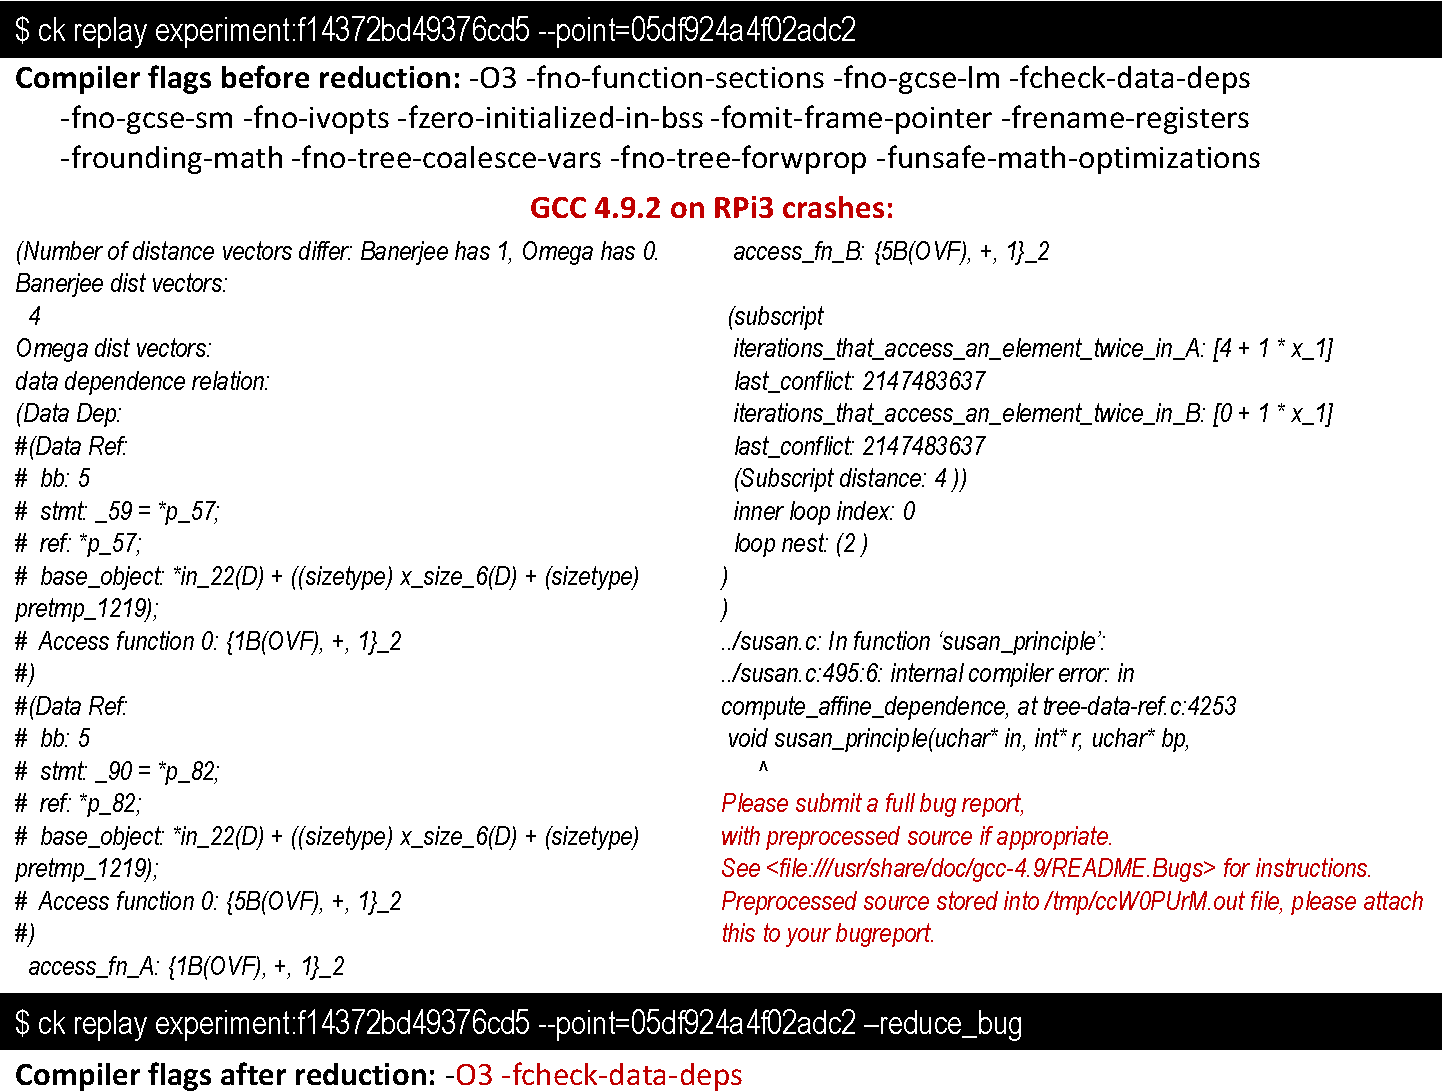
\includegraphics[width=5.2in]
      {ck-assets/60e96767e8bd4522-cropped.pdf} %CK_URL={60e96767e8bd4522-cropped.pdf}
     \caption{
       Basic example of reproducing and reducing GCC bugs after random compiler flag autotuning.
     }
     \label{fig:ck-trivial-fuzzing-example}
   \end{figure*}

Figure~\ref{fig:ck-trivial-fuzzing-example} shows a simple example of reproducing 
a GCC bug using CK together with the original random combination of flags 
and the reduced one.
%
GCC flag \emph{-fcheck-data-deps} compares several passes for dependency analysis
and report a bug in case of discrepancy.
%
Such discrepancy was automatically found when autotuning \emph{susan corners} 
using \emph{GCC 4.9.2} on RPi3.

Since CK automatically adapts to a user environment, it is also possible
to reproduce the same bug using a different compiler version.
%
Compiling the same program with the same combination of flags on the same platform
using \emph{GCC 7.1.0} showed that this bug has been fixed in the latest compiler.

We hope that our extensible and portable benchmarking workflow will help students and engineers 
prototype and crowdsource different types of fuzzers.
It may also assist even existing projects~\cite{microsoft-fuzz,oss-fuzz}
to crowdsource fuzzing across diverse platforms and workloads.
For example, we collaborate with colleagues from Imperial College London
to develop CK-based, continuous and collaborative OpenGL and OpenCL compiler 
fuzzers~\cite{Lidbury:2015:MCF:2737924.2737986,DBLP:journals/corr/LascuD15,ck-clsmith}
while aggregating results from users in public or private repositories 
(~\href{http://cknowledge.org/repo/web.php?template=cknowledge&wcid=bc0409fb61f0aa82:1b437e72c74fe782&table_sort=2}{link to public OpenCL fuzzing results across diverse desktop and mobile platforms}).

\textit{All scripts to reproduce experiments from this section are available in the following CK entry:}

\begin{flushleft}
\texttt{\$ ck find script:rpi3-susan-fuzz-bugs}
\end{flushleft}
